\documentclass[11pt]{article}

\usepackage[letterpaper,margin=1in]{geometry}
\usepackage{amsmath}
\usepackage{amssymb}
\usepackage{booktabs}
\usepackage{caption}
\usepackage{float}
\usepackage{graphicx}
\usepackage[hidelinks]{hyperref}
\usepackage{microtype}
\usepackage{parskip}
\usepackage{titlesec}

\titleformat{\section}{\large\bfseries}{\thesection}{0.6em}{}
\titleformat{\subsection}{\normalsize\bfseries}{\thesubsection}{0.6em}{}
\captionsetup{font=small,labelfont=bf}

\title{\textbf{Spaceframe Topology Optimization using Machine Learning}}
\author{Khushi Kapoor \and Johnathan Clayton \and Elijah Weddle}
\date{}

\begin{document}

\maketitle

\begin{abstract}
The design of lightweight structural systems is a fundamental challenge in engineering, particularly in applications where material choices directly impact performance, such as aerospace and mechanical systems. This project investigates a machine learning-based approach to optimizing the topology and geometry of two-dimensional spaceframe structures. The objective is to generate truss configurations that satisfy static equilibrium under loading while minimizing total structural mass. Traditional topology optimization methods often struggle in scenarios where applied loads are small relative to member weight, leading to poor convergence or impractical solutions. Using a physics-informed loss function and gradient-based optimization through the Adam optimizer, the model iteratively adjusts node positions to balance equilibrium constraints while minimizing mass. The results demonstrate that this approach can generate physically consistent truss structures and reduce mass relative to initial random configurations. This work highlights the potential of machine learning as a framework for structural optimization and provides a foundation for extending these methods to more complex, real-world applications.
\end{abstract}

\section{Introduction}

In a fully optimized structure, all elements are sized to have the maximum safe stress to minimize weight. In a heavily loaded case where space is constrained, most of the volume will necessarily be taken up with material. But given a lightly loaded case, as the scale becomes larger and geometric constraints become less pressing, more efficient shapes can be achieved. As 3D printing matures, geometric constraints become less pressing because traditionally complex geometry has little penalty.

Trusses have three distinct synergies with selective laser sintering (SLS) metal 3D printing. Due to the higher strength of 3D printed metal compared to polymer 3D printing, many loads will be small compared to the strength of the material. SLS naturally creates circular cross sections of truss members with the laser melt and can move rapidly between truss members. Finally, lowering the weight of an SLS 3D printed component lowers its machine time, which likewise lowers its cost. Although 3D printed trusses do not have true pin joints at the connections, their moment-carrying capability is small compared to their compressive and tensile strength, making the approximation appropriate.

This project optimizes the topology of trusses in two dimensions. A network of fixed nodes, free nodes, and loaded nodes was used to calculate force equilibrium with some residual. The forces from those equilibria were used to size member diameters via Euler buckling, which defined member mass. The equilibrium residual and combined member mass were combined as physics and mass loss to obtain the overall loss function. The member forces and node positions were then optimized to reach static equilibrium and low truss weight.

This optimization process benefits from the truss simplification, as strengthening relevant connections and deactivating less useful ones is exactly what these optimizers are built to do in neural networks. The truss takes the form of a fully connected graph network, with the exception that some nodes are also free to move position. The truss neural network trained through this optimization process yields the result directly in its network properties.

\section{Related Work}

Three papers focused on optimizing spaceframe trusses were analyzed. \emph{Topology optimization of spatial frames} by Schroeder and Cardoso used a 3D grid of points with various connections. Their method optimized the topology by trimming the less impactful nodes from the lattice, but the node positions were not allowed to move, limiting the flexibility of the solver.

\emph{Topology optimization of frame structures with stress and stability constraints} likewise used a 2D or 3D lattice of points whose connections were gradually trimmed.

\emph{Ultralight Fractal Structures from Hollow Tubes} deals with exclusively one-dimensional compression members. It solves the buckling equation to size truss members, then replaces those members with smaller trusses. Replacing the one-dimensional members in a truss solver like ours, or the solvers above, with hierarchical trusses would likely lead to even lower structure weights.

\section{Data}

There are multiple variables to account for in the data set. The problem does not have a traditional dataset to learn from. Instead, the input data consists of the locations and forces on the loaded and fixed nodes. Each individual load case is trained until convergence. With the number of nodes used in this project, this remains computationally reasonable. For larger and more complex systems, it may become beneficial to train a higher-level model using the outputs of this model as training data to decrease compute time.

\section{Methods}

There are two methods to analyze: the structural method and the optimization method. Although these two play interdependent roles, it is useful to consider them as distinct. The structural method ties in several concepts and principles taught throughout Washington University's Mechanical Engineering and Materials Science courses. The optimization method is more specific to MEMS 5205, Machine Learning Applications in Mechanical Engineering.

The structural method was intentionally kept simple. The model is limited to two-dimensional spaces, all pin connections, a predefined number of free nodes, and two fixed nodes. Given these constraints, the force balance equations become simple balances and no reaction moments need to be accounted for, since pin connections cannot counter a moment. This approach simplifies the physics and reduces run times, which is important for focusing on optimization while working on personal computers.

To analyze the optimization, the truss is modeled as a graph consisting of nodes and edges, where nodes represent joints and edges represent structural members. This representation allows the problem to be treated similarly to a neural network, where connections between nodes can be adjusted continuously during optimization. The goal of the optimization process is to identify a configuration that is both physically valid and efficient, meaning the structure must satisfy static equilibrium under applied loads while minimizing total structural mass. By framing the problem in this way, the model can evaluate how well a given truss configuration has been designed through a defined loss function, which guides the optimization process.

The total mass of the structure is computed as the sum of the masses of individual members, with each member's mass depending on both its geometry and the magnitude of the force it must carry. In the implementation, member sizing is implicitly tied to force requirements, meaning that larger internal forces lead to larger required cross-sectional areas and therefore higher mass. This relationship is derived using principles from structural mechanics, including Euler buckling, to ensure that members are sized sufficiently to avoid failure under compressive loads. A current limitation of the model is that both tension and compression members are sized via buckling, which is conservative for tension members. Unfortunately, when the difference is taken into account, the weight discontinuity around zero force breaks the gradient optimizer.

At the same time, the structure must satisfy static equilibrium, meaning that the net force at each node must be zero when accounting for both internal member forces and externally applied loads. To enforce this, the model computes force contributions from each connected member in both the x and y directions and compares the resulting sum to the external load vector at each node. The calculations designing the truss do not need to account for moments because each connection is assumed to be a pin.

These competing requirements are incorporated into a physics-informed loss function that balances equilibrium satisfaction with mass minimization. The loss function is defined as a weighted sum of two primary terms: a physics loss and a mass loss.

\begin{equation}
  \mathcal{L}_{total} = \alpha \mathcal{L}_{physics} + \beta \mathcal{L}_{mass}
\end{equation}

The physics loss measures how well the structure satisfies equilibrium by penalizing any imbalance in forces at each node. The mass loss estimates the total weight of the structure and encourages the optimizer to favor lighter designs. The relative importance of these objectives is controlled by weighting parameters $\alpha$ and $\beta$. These parameters must be selected carefully, as placing too much emphasis on mass reduction can lead to unrealistic structures that do not satisfy equilibrium, while prioritizing physics too heavily can result in unnecessarily heavy designs.

To minimize the loss function, a gradient-based optimization approach is used. Specifically, the Adam optimizer is employed due to its stable and efficient convergence. Adam improves upon standard gradient descent by incorporating both the average of past gradients and the variability of those gradients into the update step. This allows the optimization process to adaptively adjust step sizes for each variable, leading to faster convergence and improved numerical stability. In this problem, the optimizer computes how small changes in node positions and connection properties affect the total loss and then updates these variables in a direction that reduces the loss.

During each iteration, the model calculates internal forces in each member, resolves those forces into their directional components, evaluates the equilibrium residual at each node, and computes the corresponding mass contribution of each member. Based on these calculations, gradients of the loss function are determined with respect to the design variables, and the optimizer updates the structure accordingly. Over successive iterations, this process leads to a gradual refinement of the truss configuration.

\section{Experiments and Discussion}

To interpret the results quickly and visually, a plotting function was developed. The plotting function assigns a shape to fixed nodes, free nodes, and load points to distinguish the three types of nodes. To reduce the amount of plots analyzed and keep run times reasonable, the graphs plot at specific intervals, such as every 10,000 or 50,000 steps.

There are a few main features of the plotting functions that are worth noting. The plotting function assigns line thickness based on rod diameter. Seeing this visually shows not only which members bear more load, but also which members have the potential to be pruned.

\begin{figure}[H]
  \centering
  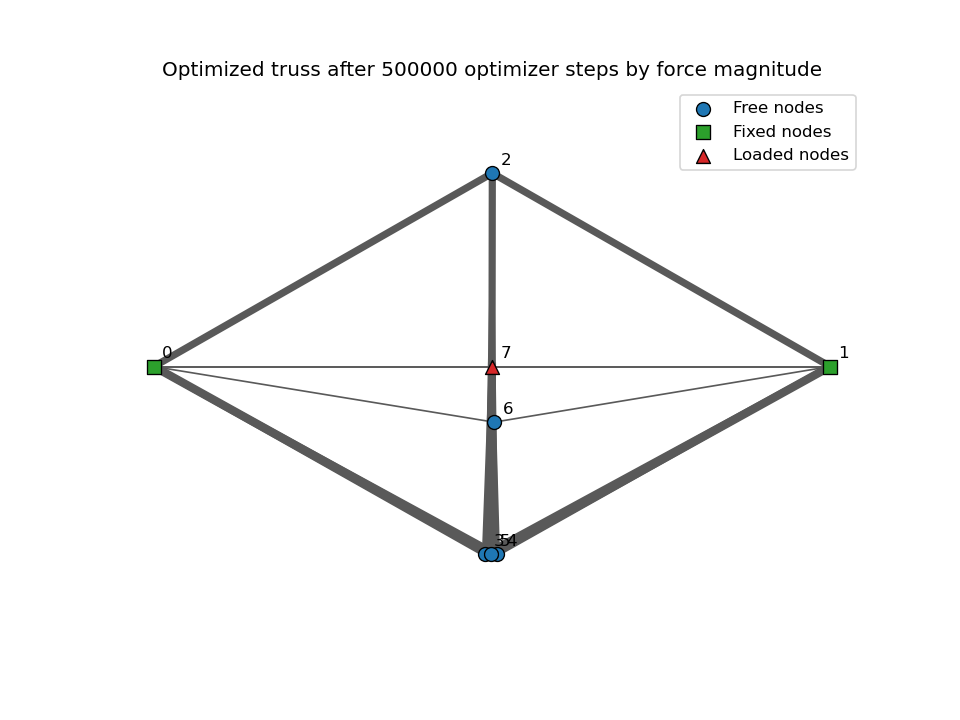
\includegraphics[width=0.82\linewidth]{../assets/optimized-bridge.png}
  \caption{Optimized bridge truss after 500,000 optimizer steps. Fixed nodes, free nodes, and loaded nodes are marked separately, and member thickness indicates force magnitude.}
  \label{fig:optimized-bridge}
\end{figure}

The beginning of the optimization causes the most noticeable and significant changes. The first 50,000 iterations cause the majority of movement in nearly every configuration of loads and supports, which matches expectations for this type of optimizing loop. Larger changes occur early, while later iterations refine the geometry and force distribution.

\begin{figure}[H]
  \centering
  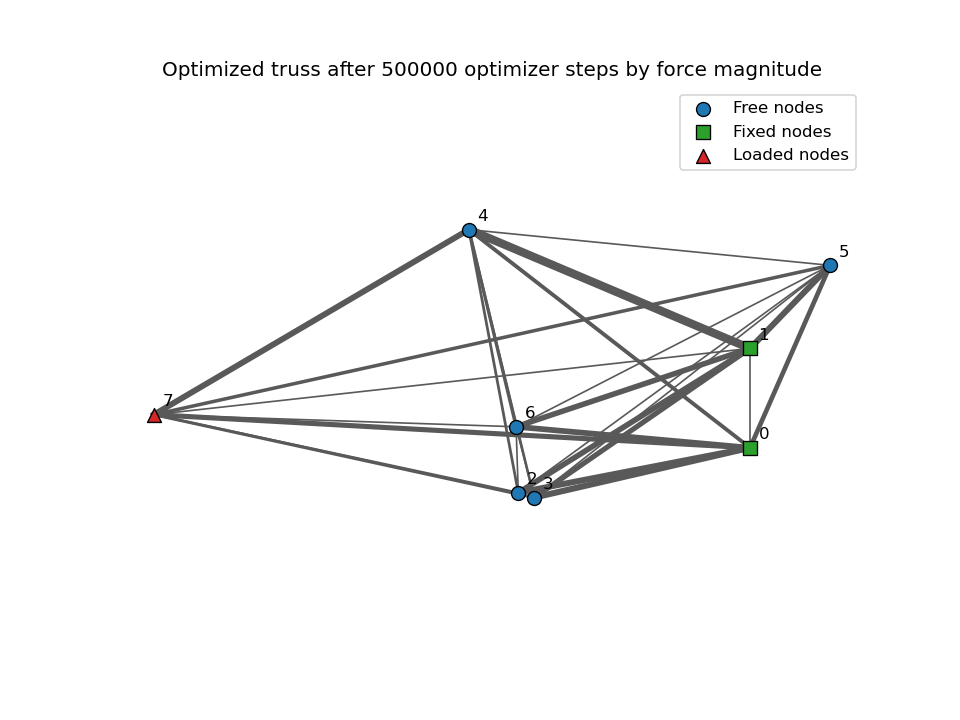
\includegraphics[width=0.74\linewidth]{../assets/cantilever-result.png}
  \caption{Optimized cantilever case showing that the same optimization framework can adapt to a different support and loading configuration.}
  \label{fig:cantilever}
\end{figure}

\subsection{Iterations and Refinements}

The physics loss and mass loss are balanced against each other, where the relative weighting changes over iterations. The physics loss weighting factor $\alpha$ decreases toward the middle of an iteration run, then ramps back up to its initial value. This enables the model to take larger geometry jumps in the middle while still ensuring that it yields an accurate result in the end. Without this changing $\alpha$, the model tends to get stuck either disregarding physics entirely or being too timid to move nodes substantially, since that will temporarily change the force balance.

To improve model performance and visual clarity, a trimming function was used to mask out members whose diameter averaged under a given threshold over several model iterations.

Several future improvements could make this tool more useful in real applications. These include implementing a 3D solver instead of a 2D solver, adding keep-out zones where the model is penalized for placing members, creating a post-processor to export OpenSCAD scripts for 3D models, adding a smoothing algorithm for intersection points, and physically accurately handling intersections between members.

\subsection{Analysis}

The loop gravitates toward traditional shapes that should be recognized by mechanical engineering and structural engineering students. The bridge-loaded simulations clearly trend toward diamond shapes built by obvious triangles, one of the strongest structural motifs.

The trend of the geometric configuration of the nodes is encouraging, but further analysis is required to determine effectiveness and success across larger design spaces, more load cases, and more realistic constraints.

\section{Conclusion}

In conclusion, the topology optimization framework developed in this project successfully demonstrated the ability to generate lightweight truss structures that satisfy static equilibrium while minimizing structural mass. By modeling the truss as a graph and applying a physics-informed loss function, the approach was able to balance competing objectives of physical validity and efficiency through gradient-based optimization. The use of the Adam optimizer allowed for stable convergence and enabled continuous updates to node positions and member properties, resulting in optimized structures that reflect recognizable and efficient engineering designs. The emergence of traditional truss geometries, such as triangular and diamond-shaped configurations, further supports the validity of the method, as these forms are known to be structurally efficient.

This work highlights the effectiveness of combining classical structural mechanics principles with modern machine learning techniques. The integration of equilibrium constraints, Euler buckling-based member sizing, and loss-based optimization provides a flexible framework that can adapt to different loading conditions and boundary configurations. Additionally, the ability of the model to start from random initial configurations and converge toward meaningful structural layouts demonstrates its potential as a generative design tool.

However, several limitations were identified throughout the project. The balance between physics loss and mass loss remains highly sensitive, and improper tuning can lead to either physically invalid structures or overly conservative designs. The use of a single sizing method for both tension and compression members introduces conservatism and limits physical realism. Furthermore, the current implementation is restricted to two-dimensional systems, which reduces its applicability to real-world engineering problems. Computational cost is also a significant challenge, as extending the model to more complex systems or higher node counts would require substantially more processing power.

Future work should focus on extending the framework to three-dimensional spaceframes, which would significantly increase its practical relevance. Incorporating more accurate material models, including separate treatment of tension and compression members, would improve physical fidelity. Additional constraints such as stress limits, buckling modes, and manufacturability considerations could also be integrated into the loss function. From a machine learning perspective, developing adaptive weighting strategies for the loss terms or training a higher-level model to predict optimized configurations could improve convergence speed and robustness. Improvements to pruning strategies and post-processing techniques would also help produce cleaner and more realistic final designs.

Overall, this project demonstrates that machine learning provides a promising and flexible approach to structural topology optimization. While further refinement is needed, the results establish a strong foundation for future development and highlight the potential for combining physics-based modeling with data-driven optimization techniques in engineering design.

\section*{Contributions}

Johnathan Clayton developed functions for distance calculation, physics-loss node sums, mass loss, total loss, and moving averages. He also implemented trimming behavior, time-varying $\alpha$ and $\beta$ values, and contributed to future-improvement framing and the project introduction.

Elijah Weddle spearheaded LaTeX integration, wrote code for visualizing optimization results, and wrote and presented the data and results sections.

Khushi Kapoor wrote code to calculate diameter and weight using inputs such as force, length, and Young's modulus. She helped implement and test mass and physics loss functions, wrote and presented the methods section, and wrote the abstract and conclusion.

\begin{thebibliography}{9}

\bibitem{schroeder2024}
Schroeder, W. and Cardoso, E. \emph{Topology optimization of spatial frames}. 2024.

\bibitem{stressstability2022}
\emph{Topology optimization of frame structures with stress and stability constraints}. 2022.

\bibitem{fractal2012}
Fleck, N. A., Deshpande, V. S., and Ashby, M. F. \emph{Ultralight Fractal Structures from Hollow Tubes}. Physical Review Letters, 2012.

\end{thebibliography}

\end{document}
